%
% Vector table
%
\documentclass[border=3mm]{standalone}
\usepackage{tikz}
\usetikzlibrary{circuits.ee.IEC}

\begin{document}

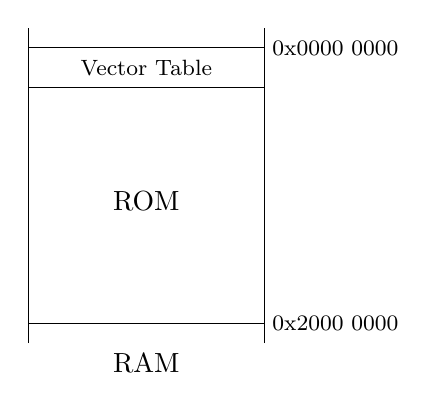
\begin{tikzpicture}
    \draw [-] (0,0) to (0,4);
    \draw [-] (3,0) to (3,4);
    \draw [-] (0,0.25) to (3,0.25);
    \draw [-] (0,3.75) to (3,3.75);     % ROM start
    \draw [-] (0,3.25) to (3,3.25);     % Vector end
    \node (rom_start) at (3.1,3.75) {};
    \node (ram_start) at (3.1,0.25) {};
    \node (rom) at (1.50,-0.25) {RAM};
    \node (ram) at (1.50,1.80) {ROM};
    \node (heap) [font=\footnotesize] at (1.50,3.50) {Vector Table};
    \node [font=\footnotesize,right] at (rom_start.west) {0x0000 0000};
    \node [font=\footnotesize,right] at (ram_start.west) {0x2000 0000};
\end{tikzpicture}

\end{document}

